\documentclass{hwz}
% \usepackage{showframe}
\usepackage{lipsum}

\begin{document}

%#############################
% Title page
%#############################
\makeTitlepage{Automatisierung von Kundenservices durch künstliche Intelligenz am Beispiel der Rückforderungseinreichung in der Krankenversicherung}{Dr. Oliver Zenklusen}{Sven Tschui}{15-522-345}{BWI-A15}{Winterthur, 2. Mai 2019}

%#############################
% Abstract
%#############################
\makeAbstract{Management Summary}{
    \lipsum[4]
}

\newpage

%#############################
% Table of contents
%#############################
\tableofcontents

\newpage

%#############################
% Declaration of authorship
%#############################
\makeDeclarationOfAuthorship{Winterthur}{2. Mai 2019}{Sven Tschui}

\newpage

%#############################
% Preface
%#############################
\makePreface{Vorwort}{
    \lipsum[3]
}

\newpage


%#############################
% Intro
%#############################
% This will add roman page numbering and page header from here on
\makeBeginMain
\section{Einleitung}

\lipsum[2]

\newpage

%#############################
% Section #1
%#############################
\section{Lorem ipsum}

\lipsum[2]

\enquote{This is a direct citation}~\autocite{Nadeau2007AClassification}. And some more text.

This is a paraphrased citation \autocite{Nadeau2007AClassification}.

\lipsum[1]

\begin{figure}[h]
\caption{Example of a parametric plot ($\sin (x), \cos(x), x$)}
\centering
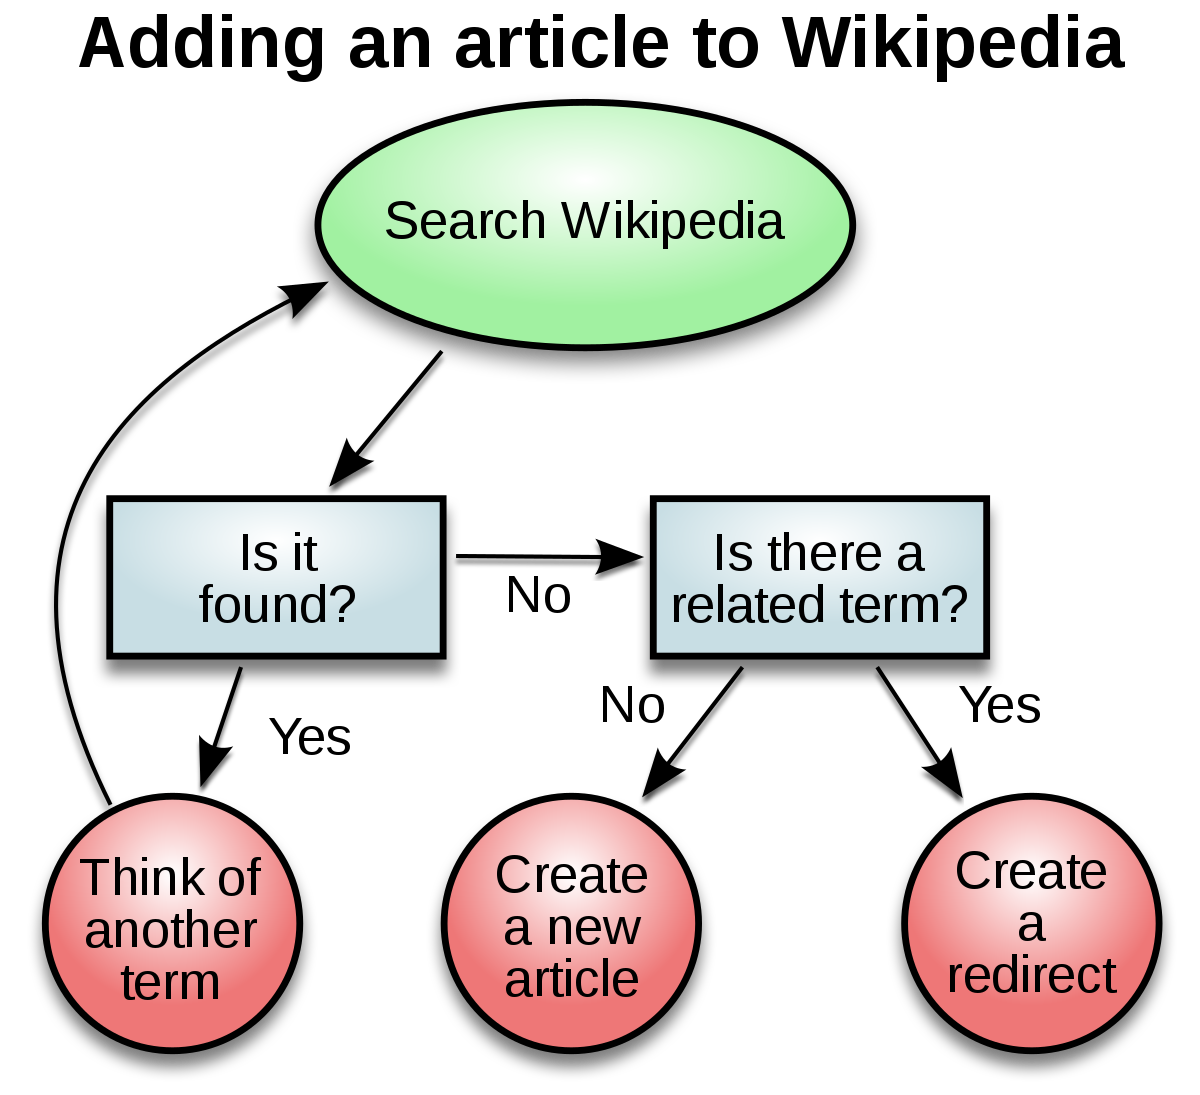
\includegraphics[width=0.5\textwidth]{graphics/wikipedia.png}
\caption*{Quelle: \textcite{BundesamtfurStatistik2018Finanzierung}}
\end{figure}

\lipsum[2]

\begin{table}[h]
\centering
\caption{Table to test captions and labels}
\label{table:1}
\begin{tabular}{||c c c c||} 
 \hline
 Col1 & Col2 & Col2 & Col3 \\ [0.5ex] 
 \hline\hline
 1 & 6 & 87837 & 787 \\ 
 2 & 7 & 78 & 5415 \\
 3 & 545 & 778 & 7507 \\
 4 & 545 & 18744 & 7560 \\
 5 & 88 & 788 & 6344 \\ [1ex] 
 \hline
\end{tabular}
\caption*{Quelle: \cite{BundesamtfurStatistik2018Finanzierung}*}
\end{table}
\newpage

%#############################
% Sub-Section #1.1
%#############################
\subsection{Sub-section Lorem ipsum}

% TODO: Text here
\lipsum[2]

\newpage

%#############################
% Section #2
%#############################
\section{Lorem ipsum 2}

% TODO: Text here
\lipsum[2]

\newpage

%#############################
% Appendix
%#############################
\section{Anhang}

\makeBibliography{Anhang}{Literaturverzeichnis}

\newpage

\makeListOfTablesAndFigures{Tabellen- und Abbildungsverzeichnis}

\end{document}